Major Trauma Management is among the most challenging scenarios in the healthcare context due to its time-dependent nature.
%
This use case has been used in several works~\cite{web-of-dt-ricci-2022,Croatti_Gabellini_Montagna_Ricci_2020,Montagna2019} to demonstrate how \acp{DT} can support the complex processes involved in trauma care.
%
Timely diagnosis, identification, and response are paramount in ensuring patient health. The entire process has been divided into three main stages:
\begin{enumerate}
    \item \emph{Emergency Call Management}, where the \ac{CEU} receives, plans, and initiates a first-aid emergency mission;
    \item \emph{Pre-Hospital Management}, which encompasses the time from the rescuer's initial assessment and treatment to the patient's transfer to the trauma center; and
    \item \emph{Trauma Management}, which includes all the processes undertaken by the trauma team in the trauma center to preserve the patient's life.
\end{enumerate}
%
A recent solution presented in \cite{Montagna2019} already deeply investigates the latter stage. 
Hence, this chapter is dedicated to the design and implementation of a \acp{DTE} for the \emph{Emergency Call} and the \emph{Pre-Hospital Management} stages of trauma management.
%
This case study is used to demonstrate how the \ac{HWoDT} framework (\Cref{chap:dte:hwodt}) can be employed to integrate heterogeneous \acp{DT} from different systems into a coherent ecosystem, enabling interoperability and advanced functionalities across the entire trauma management process.


%=======================================================
\section{Case Study Analysis}
%=======================================================

A detailed analysis of the case study is provided in \cite{web-of-dt-ricci-2022}.
%
Here main aspects are summarized to provide context for the \acp{DTE} proposal and introduce the terminology. 

The typical scenario begins when a \ac{CEU} operator receives an emergency call.
The operator gathers the \emph{event} first-contact information and initiates a new \emph{mission} for each victim involved.
An \emph{ambulance} and a designated \emph{rescuer} are then assigned to each mission to reach the patient and provide first aid.
%
Upon arrival, the emergency crew establishes contact with the \emph{patient}, who may be identified as an authorized \emph{healthcare user} by the health insurance card. According to their conditions, a destination \emph{trauma center} is selected. The patient is continuously monitored during the whole process, especially while establishing a \emph{diagnosis}.

A variety of departments must interact within the context of a complex operational environment, as is the case in the healthcare domain. In order to accomplish their responsibilities, each of them exploits a range of systems that may be developed with different technological stacks due to the fragmented evolution of electronic health systems (e.g., legacy, subcontractors).
%
In the context of this scenario, two principal responsibilities can be identified. The first is the management of emergency calls, which includes the resources planning for missions. The second is the pre-hospital management of the ongoing trauma.

For this hypothetical case study, both systems are assumed to be implemented with a \ac{DT}-based rationale, using different technologies.
%
Namely, the prototype \acp{DTE} is constructed assuming that
\acl{WLDT} is used for emergency call management and planning, while \azureTwin{} is used for pre-hospital management. Finally, Eclipse Ditto has been employed to represent the Healthcare User \ac{DT}, to simulate an external data source, typically the National Health Service.

%=======================================================
\section{\acl{DTE} Proposal}
%=======================================================

\begin{figure}
  \centering
  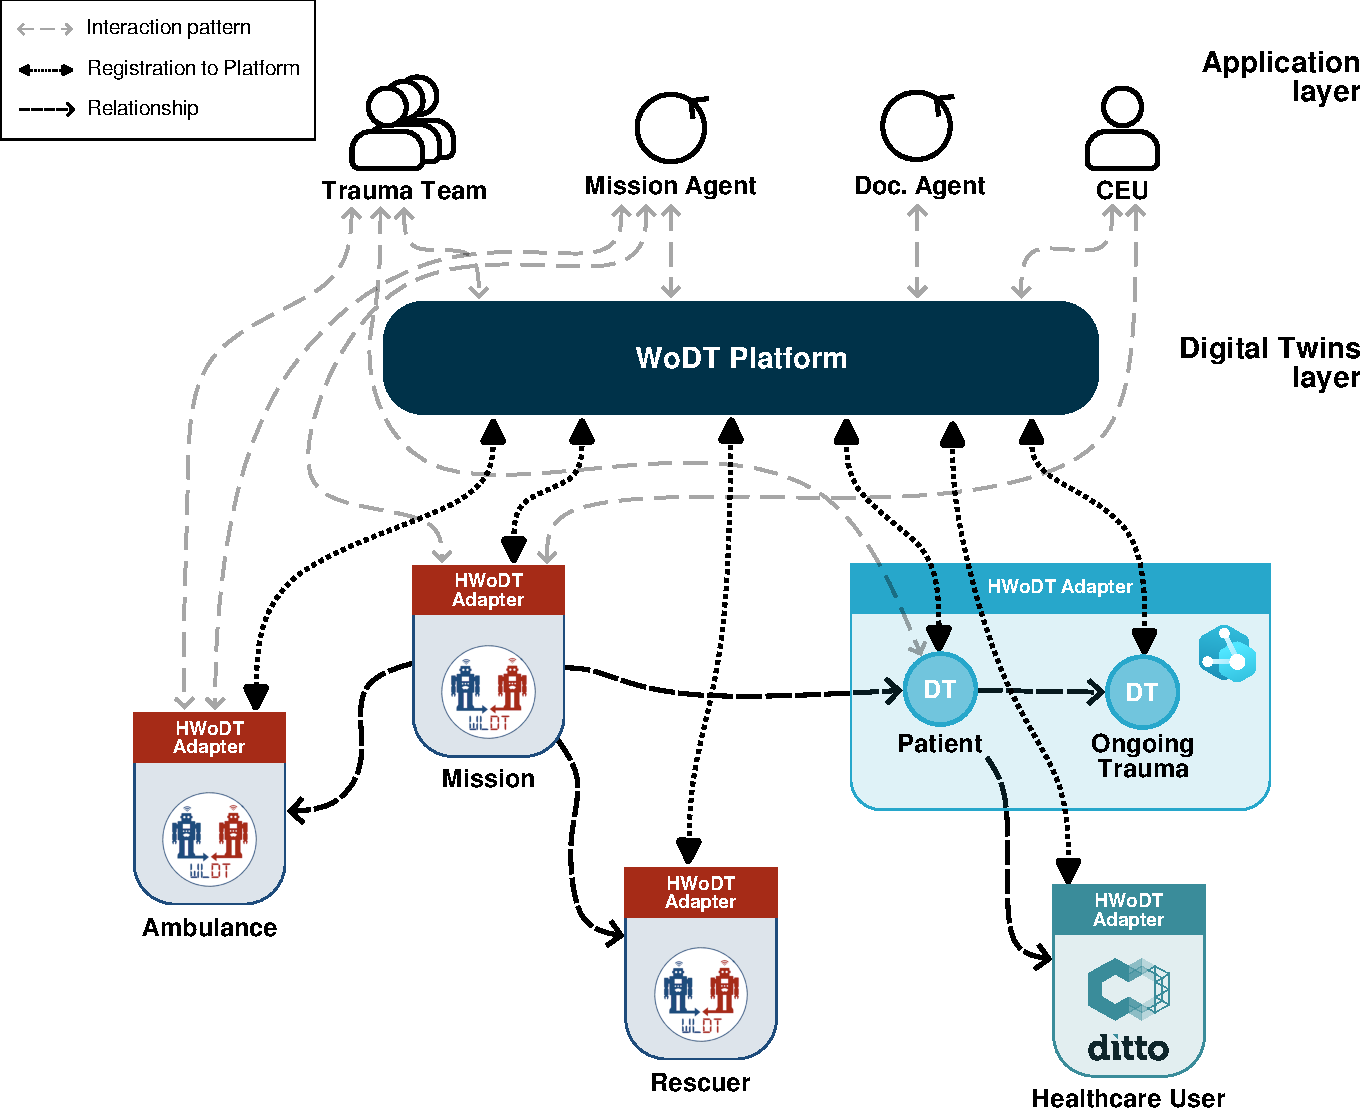
\includegraphics[width=\columnwidth]{figures/hwodt/major-trauma-management.pdf}
  \caption{The \ac{HWoDT}-based \ac{DTE} for the trauma management case study. \acp{DT} implemented with different technologies (WLDT, Ditto, Azure) become interoperable through the HWoDT Adapters and are integrated through the WoDT Platform. 
  Black dotted arrows represent the interaction with the platform, black dashed arrows represent relationships between \acp{DT} while grey arrows represent the interaction between consumers, the platform and \acp{DT}.
  }
  \label{fig:trauma-use-case-diagram}
\end{figure}

Figure \Cref{fig:trauma-use-case-diagram} illustrates the envisioned \ac{HWoDT}-based \ac{DTE} for the trauma management use case.
%
\acp{DT} of different entities are modeled: 
\begin{itemize}
    \item \emph{Mission} \ac{DT}, representing the emergency mission, to track the state of the mission as the process goes on, implemented with \ac{WLDT};
    \item \emph{Ambulance} \ac{DT}, representing the ambulance vehicle, allowing to monitor its location and availability, implemented with \ac{WLDT};
    \item \emph{Rescuer} \ac{DT}, representing the medical staff member that can be assigned to a mission, again allowing to monitor availability and qualification, implemented with \ac{WLDT};
    \item \emph{Patient} \ac{DT}, representing the patient being rescued. This \ac{DT} represents the patient in the hospital system and can be used to collect medical documentation about the patient from as soon as the medical team arrives at site and starts monitoring vital signs, implemented with \azureTwin{};
    \item \emph{Ongoing Trauma} \ac{DT}, representing the trauma being managed, used to track the state of the process from a medical perspective, and continuing even after the mission is closed at the hospital, implemented with \azureTwin{};
    \item \emph{Healthcare User} \ac{DT}, representing the patient's healthcare profile in a national external record to access its clinical history, implemented with Eclipse Ditto.
\end{itemize}


%=======================================================
\section{Implemented Solution}
%=======================================================

Each \ac{DT} is mapped to the \ac{HWoDT} uniform interface through the respective adapter, enabling interoperability within the ecosystem.

The \ac{WoDT} platform is deployed to provide ecosystem services, including the \ac{DTE} \ac{KG}, which integrates data from all \acp{DT} using the HL7 FHIR standard to represent healthcare resources.

The trauma management process is supported by the \ac{DTE} as follows:
\begin{enumerate}
    \item When the \emph{CEU operator} receives an emergency call, it collects the first-contact information and, according to the rescue process, a \emph{Mission \ac{DT}} is instantiated for each mission.
    \item Upon receiving the \ac{URI} of a new Mission \ac{DT}, the \emph{Mission Agent} -- a software for supporting the automatic allocation of resources -- is responsible for identifying free resources, namely a \emph{rescuer} and an \emph{ambulance}, to assign to the mission. The \emph{Mission Agent} requires a comprehensive and updated view of the current state of the \ac{DTE}. In order to identify an inactive ambulance and an available rescuer with the right qualification (Paramedic), the SPARQL query described in \Cref{lst:ambulance-rescuer-query} is executed on the \ac{WoDT} Platform. 

    \begin{code}
    \captionof{listing}{SPARQL Query performed by the Mission Agent to obtain the available ambulances and rescuers.}
    \label{lst:ambulance-rescuer-query}
    \inputminted{sparql}{listings/hwodt/use-case/ambulance-rescuer-query.rq}
    \end{code}
    
    \item The resources are allocated to the mission. The relationships with the identified \emph{Ambulance} and \emph{Rescuer \acp{DT}} are updated by the shadowing process of the involved \ac{DT}.
    \item The \emph{Mission Agent} controls the ambulance onboard system setting the destination to reach. It obtains the Ambulance \ac{DTD} (\Cref{lst:ambulance-dtd}), fetches the interaction affordance of the \texttt{SetDestinationCommand} action, and performs a request to it.

    \lstinputlisting[
        caption={Portion of the Ambulance \ac{DTD} that shows the relevant data for the \texttt{SetDestinationCommand} action},
        label={lst:ambulance-dtd},
    ]{listings/hwodt/use-case/ambulance-dtd.json}    


    \item When the ambulance reaches the patient, a new \emph{Patient \ac{DT}}, is created to track their health status. A relationship is established between the Mission \ac{DT} and the Patient \ac{DT}. The resulting Mission \ac{DTKG} is reported in \Cref{lst:mission-dtkg}.

    \begin{code}
    \captionof{listing}{The Mission \ac{DTKG} when the ambulance reaches the patient, showing the relationship with the patient.}
    \label{lst:mission-dtkg}
    \inputminted{turtle}{listings/hwodt/use-case/dtkg-missiondt.ttl}
    \end{code}
    
    Meanwhile, the patient's tax code, if available, is collected and the associated \emph{Healthcare User \ac{DT}} is discovered via the Platform DT Discovery Service. This service, starting from a \ac{PA} identifier, returns the corresponding \acp{DT} within the ecosystem. Subsequently, a relationship is established with the Patient \ac{DT}.
    \item The trauma team is informed about the imminent arrival of the patient by receiving the Mission \ac{DT} \ac{URI}. In order to prepare to handle the incoming patient, they can observe the incoming patient and the ambulance \acp{DT}.
    %
    The aggregation of \acp{DTKG} and \acp{DTD} on the \ac{WoDT} Platform is exploited to obtain both interaction affordances by executing the SPARQL query described in \Cref{lst:patient-ambulance-observation-endpoints-query}. The returned affordances are then used to observe the respective \acp{DT}.

    \begin{code}
    \captionof{listing}{SPARQL Query performed by the trauma team support tools to obtain the ambulance and patient observation endpoints.}
    \label{lst:patient-ambulance-observation-endpoints-query}
    \inputminted{sparql}{listings/hwodt/use-case/patient-ambulance-observation-endpoints-query.rq}
    \end{code}
    
    
    \item Finally, the \emph{OnGoingTraumaDT} is created to collect information on the trauma process supporting the trauma management stage.
\end{enumerate}

On top of \acp{DT} and \ac{WoDT} Platform, the business logic and automated control of the scenario are implemented through different applications:

\begin{itemize}
    \item The aforementioned \emph{Mission Agent}, which observes the \ac{DTE} \ac{KG} and manages new missions by assigning resources.
    \item The \emph{Documentation Agent}, which observes the \ac{DTE} \ac{KG} for the automatic generation of the trauma documentation (cfr. TraumaTracker~\cite{Montagna2019}).
    \item The \emph{\ac{CEU} Dashboard} periodically monitors the currently active missions by executing the SPARQL query in \Cref{lst:active-missions-query}.

    \begin{code}
    \captionof{listing}{SPARQL Query performed by the \ac{CEU} Dashboard to obtain the currently active missions.}
    \label{lst:active-missions-query}
    \inputminted{sparql}{listings/hwodt/use-case/active-missions-query.rq}
    \end{code}
    
\end{itemize}


%=======================================================
\section{Discussion}
%=======================================================

The demonstration of the implementation and exploitation of a \ac{HWoDT} ecosystem through the use case of trauma management, allows showcasing the potential benefits of the proposed approach from a practical perspective.
%

As already discussed in \Cref{sec:dte:hwodt:related}, this approach allows to integrate heterogeneous \acp{DT} implemented with different technologies under a uniform interface. 
%
This further enhances the decoupling of applications from the underlying technologies, further supported by the explicit semantic layer that hides the concrete implementation of the individual \acp{DT}.
%
Applications exploiting the \ac{DTE} can be programmed using Web technologies. This eases the creation of supporting dashboards and automation tools (i.e. the \emph{Mission Agent}) since the \acp{DT} are exposed as Web resources.
%
Without the \ac{HWoDT} this would much harder, as each \ac{DT} may expose different \ac{API} and maintaining the functionalities of the application would require dealing with the fragmented evolution of the underlying systems.

As a result, application developers can focus solely on the application logic, abstracting away the complexity of diverse \ac{DT} technology APIs and SDKs. 
This approach yields two key advantages:
\begin{itemize}
    \item a more stable \textbf{application layer}, which remains unchanged when new \ac{DT} technologies are introduced, thereby simplifying the integration of additional organizations and stakeholders; and
    \item a more stable \textbf{\ac{DT} layer}, which can evolve or replace underlying technologies without impacting the upper layers, thanks to effective information encapsulation and technology hiding.
\end{itemize}

Additionally, the scenario demonstrates the advantages of tracking relationships between \acp{DT} which in this application are crucial to understand the context of each entity involved in the trauma management process and monitor the overall state of ongoing processes effectively.
%
In this scenario, new \acp{DT} tracking process state are created dynamically when needed (i.e., Mission \ac{DT}, Patient \ac{DT}, OngoingTrauma \ac{DT}), and relationships are established among them to represent their interactions and dependencies.
%
This would be very hard to achieve without an explicit notion of \ac{DTE}, and the functionalities the abstraction can serve (e.g., discovery, navigation, querying, observation). 


Being based on the notion of a \ac{KG}, the resulting \ac{DTE} can benefit from the explicit semantic representation of entities and concepts, allowing powerful and expressive queries to find information on the state of the ecosystem.
%
Of course, this requires an additional effort when developing (or mapping) \acp{DT}, as the appropriate domain ontologies need to be used to represent the knowledge provided by \acp{DT}.
%
In this example, we use the HL7 FHIR standard to unify healthcare data coming from different sources. This greatly improves the quality of the information generated by the \ac{DT} ecosystem.
%
We then see this effort as a valuable trade-off for the benefits it can bring to the overall ecosystem.
